\documentclass[11pt]{article}

% ---------- Packages ----------
\usepackage[margin=1in]{geometry}
\usepackage{amsmath,amssymb}
\usepackage{graphicx}
\graphicspath{{../Code/results/}}
\usepackage{booktabs}
\usepackage{longtable}
\usepackage{array}
\usepackage[table]{xcolor}
\usepackage{xurl}
\usepackage{hyperref}
\usepackage{caption}
\usepackage{enumitem}
\usepackage{fancyhdr}
\usepackage{titlesec}
\usepackage[most]{tcolorbox}

\hypersetup{colorlinks=true, linkcolor=blue!50!black, urlcolor=blue!50!black}

\definecolor{assumedcolor}{RGB}{178,34,34}
\definecolor{paolacolor}{RGB}{0,102,51}
\newcommand{\PAOLA}{\textcolor{paolacolor}{\textbf{[PAOLA]}}}
\newcommand{\ASSUMED}{\textcolor{assumedcolor}{\textbf{[ASSUMED]}}}

\newcommand{\usd}{USD}
% firm subscripts, written out so no one has to decode a letter
\newcommand{\gas}{\mathrm{Gas}}
\newcommand{\ccs}{\mathrm{CCS}}
\newcommand{\strap}{\mathrm{STRAP}}
\newcommand{\inc}{\mathrm{Inc}}

\setlength{\headheight}{14pt}
\pagestyle{fancy}
\fancyhf{}
\fancyhead[L]{\small Four recycling technologies competing for feedstock}
\fancyhead[R]{\small\thepage}
\renewcommand{\headrulewidth}{0.4pt}

\titleformat{\section}{\normalfont\Large\bfseries}{\thesection}{0.8em}{}
\titleformat{\subsection}{\normalfont\large\bfseries}{\thesubsection}{0.8em}{}
\setlength{\parskip}{0.55em}
\setlength{\parindent}{0pt}

\tcbset{
  boxsep=2pt, left=8pt, right=8pt, top=6pt, bottom=6pt,
  colback=blue!4!white, colframe=blue!50!black, fonttitle=\bfseries,
  breakable
}
\newtcolorbox{readbox}[1][]{colback=green!5!white, colframe=green!40!black,
  title={Interpretation}, unbreakable, #1}
\newtcolorbox{cautionbox}[1][]{colback=orange!7!white, colframe=orange!70!black,
  unbreakable, #1}

\title{\textbf{Competition for Feedstock Among Four\\
Plastic-Recycling Technologies}\\[0.4em]
\large A generalized Nash equilibrium model of gasification, gasification with
CCS, STRAP and incineration}
\author{Parth Brahmbhatt --- Avraamidou Lab}
\date{\today}

\begin{document}
\maketitle

% =============================================================================
\section{Introduction}
\label{sec:intro}

\subsection{The problem}

The multilayer-film decision-support paper treats waste management as a
\emph{planning} problem: one decision maker has a fixed amount of post-industrial
multilayer film and chooses how much to send to each treatment route so as to
maximize total profit. That model answers ``what is the best allocation?'' It
does not say what the waste is \emph{worth}, and it does not describe a market,
where each treatment plant is run by a separate firm that buys waste to maximize
its own profit.

This report studies that market. Four technologies compete for the same limited
supply of waste:
\begin{itemize}[leftmargin=1.6em,itemsep=0.1em]
  \item \textbf{Gasification}, producing hydrogen;
  \item \textbf{Gasification + CCS}, the same process with carbon capture, which
        earns the U.S.\ Section~45Q carbon-capture tax credit;
  \item \textbf{STRAP}, the solvent-based recycling process for multilayer film
        (its residue is landfilled);
  \item \textbf{Incineration}, with energy recovery.
\end{itemize}
Every ton one firm buys is a ton the others cannot have. The central question is:
\emph{what price does competition put on a ton of waste, who ends up buying it, what
does this depend on, and does each plant earn back its capital?}

\subsection{Approach}

We model the firms as players in a \emph{generalized Nash equilibrium problem}
(GNEP): each firm maximizes its own profit, but all firms share one constraint, the
total waste available. We compute the \emph{variational equilibrium}, in which all
firms face the same price on the shared constraint. That price, called $\lambda$
(USD per ton), is the main output. It is not assumed; it is the shadow price of the
shared waste constraint. Each firm's profit includes its annualized capital charge,
and we report whether each plant covers it.

\subsection{Summary of results}

For a base case of 20{,}000 t/yr of waste (Section~\ref{sec:results}):
\begin{itemize}[leftmargin=1.6em,itemsep=0.2em]
  \item The equilibrium price is $\lambda=932.96$ \usd/ton, and \textbf{STRAP} sets it.
  \item Gasification + CCS and Gasification each take their full 8{,}000 t/yr, and
        STRAP takes the remaining 4{,}000 t/yr (half its capacity). Incineration
        takes nothing.
  \item With the 45Q credit (270 \usd/t), Gasification + CCS earns almost exactly
        the same margin as plain Gasification (1{,}410.77 against 1{,}410.00): the
        credit offsets the extra 269 \usd/t of capture cost. The two are effectively
        tied.
  \item \textbf{STRAP does not earn back its capital at this pool size.} It runs half
        empty and loses 2.58 million \usd/yr after its annualized capital; it needs
        to process 6{,}768 t/yr (85\% of capacity) to break even. Both gasification
        plants cover their capital.
  \item The price is a staircase in the amount of waste: five values, switching at
        8{,}000, 16{,}000, 24{,}000 and 36{,}800 t/yr. The base case sits
        4{,}000 t/yr inside each edge of its step.
  \item At the base case the price depends one-for-one on STRAP's own revenue and
        operating cost, on the feedstock price and on the plant capacities, and
        not on the other firms' numbers (within wide limits).
\end{itemize}

\subsection{Conventions}

Every input is tagged \PAOLA\ (number supplied by Paola) or \ASSUMED\ (our default,
to be confirmed). Each result is followed by a green \textbf{Interpretation} box
that says in plain words what it means. Orange boxes mark something that could
change a conclusion. The questions for Paola are collected in
Section~\ref{sec:questions}.

% =============================================================================
\section{Method}
\label{sec:method}

\subsection{Setting and notation}

Let $\mathcal I=\{\gas,\ccs,\strap,\inc\}$ be the set of firms. All economic
quantities are per ton of feedstock and constant in the amount processed (linear
cost), as supplied by Paola.

\begin{table}[h]
\centering
\caption{Notation.}
\label{tab:notation}
\small
\renewcommand{\arraystretch}{1.2}
\begin{tabular}{@{}>{\raggedright\arraybackslash}p{2.4cm}>{\raggedright\arraybackslash}p{12.5cm}@{}}
\toprule
\textbf{Symbol} & \textbf{Meaning} \\
\midrule
$q_i$ & Tons per year of waste bought and processed by firm $i$ (decision variable). \\
$\mathrm{Cap}_i$ & Plant capacity of firm $i$, t/yr: the most it can process. \\
$r_i$ & Revenue of firm $i$ per ton of feed, \usd/t. For the CCS firm it includes the 45Q credit. \\
$a_i$ & Operating cost of firm $i$ per ton of feed, \usd/t. \\
$\mathrm{ACC}_i$ & Annualized capital charge of firm $i$, \usd/yr. \\
$p_{\mathrm{raw}}$ & Price the waste generator charges per ton (0 in the base case). \\
$m_i$ & Net margin of firm $i$: $m_i=r_i-a_i-p_{\mathrm{raw}}$, \usd/t. The most firm $i$ can pay for one more ton and still break even on operations. \\
$Q_{\mathrm{tot}}$ & Total waste available, t/yr. \\
$\lambda$ & Multiplier of the shared waste constraint, \usd/t: the equilibrium price of waste. \\
$\mu_i$ & Multiplier of firm $i$'s capacity constraint, \usd/(t/yr): the gain in firm $i$'s operating profit per extra ton/yr of its own capacity. \\
\bottomrule
\end{tabular}
\end{table}

\subsection{Each firm's problem}

Firm $i$ chooses $q_i$ to maximize its profit after capital
\begin{equation}
\max_{q_i\ge 0}\ \ \pi_i = m_i\,q_i-\mathrm{ACC}_i
\qquad\text{s.t.}\qquad q_i\le \mathrm{Cap}_i,
\qquad
\sum_{j\in\mathcal I} q_j \le Q_{\mathrm{tot}} .
\label{eq:firm}
\end{equation}
The last constraint is the same for all firms: it is the shared supply of waste.
Because it involves every firm's decision, this is a \emph{generalized} Nash
game and not an ordinary one. The capital charge $\mathrm{ACC}_i$ is in the
objective, but it is a constant: it does not depend on $q_i$, so it does not change
the optimal throughput. It shifts profit, and it is what we use to decide whether a
plant pays back (Section~\ref{sec:viab}).

\subsection{Equilibrium concept}

We solve for the \emph{variational equilibrium}: the equilibrium in which every
firm attaches the same multiplier $\lambda$ to the shared constraint. This is the
natural concept for a market with one clearing price, and it is the one for which
$\lambda$ can be read as ``the price of waste''. Attach $\mu_i\ge0$ to
$q_i\le\mathrm{Cap}_i$ and $\lambda\ge0$ to the shared constraint. Stacking the
optimality (KKT) conditions of all four firms gives
\begin{align}
0 \le q_i &\;\perp\; \lambda+\mu_i-m_i \ge 0, \label{eq:kkt1}\\
0 \le \mu_i &\;\perp\; \mathrm{Cap}_i-q_i \ge 0, \label{eq:kkt2}\\
0 \le \lambda &\;\perp\; Q_{\mathrm{tot}}-\textstyle\sum_{j} q_j \ge 0 ,\label{eq:kkt3}
\end{align}
for all $i\in\mathcal I$. The notation $x\perp y$ means $xy=0$. The term
$\lambda+\mu_i-m_i$ in~\eqref{eq:kkt1} does not depend on $q_i$. That is the
formal statement that cost is linear, and it drives everything below.

\subsection{Solution}

\textbf{Best response.} By~\eqref{eq:kkt1}--\eqref{eq:kkt2}, each firm's best
response to a price $\lambda$ is a step:
\begin{equation}
q_i(\lambda)=
\begin{cases}
\mathrm{Cap}_i & \text{if } m_i>\lambda,\\
0 & \text{if } m_i<\lambda,\\
\text{any value in }[0,\mathrm{Cap}_i] & \text{if } m_i=\lambda .
\end{cases}
\label{eq:br}
\end{equation}
A firm that earns more per ton than the price wants as much as its plant can
process, and a firm that earns less wants none.

\textbf{Aggregate demand and the price.} Total demand at price $\lambda$ is the
step function $D(\lambda)=\sum_{i:\,m_i>\lambda}\mathrm{Cap}_i$. By~\eqref{eq:kkt3}
the equilibrium price is the lowest price at which demand fits the supply:
\begin{equation}
\lambda^\ast=\min\{\lambda\ge0:\ D(\lambda)\le Q_{\mathrm{tot}}\}.
\label{eq:lambda}
\end{equation}
Firms strictly above $\lambda^\ast$ run at capacity, firms strictly below take
nothing, and a firm exactly at $\lambda^\ast$ takes whatever is left. At the exact
thresholds where $D$ steps, any price between two adjacent steps is consistent
with equilibrium; \eqref{eq:lambda} picks the lowest and we report that.

\textbf{Closed form (merit order).} Sort the firms by margin,
$m_{(1)}>m_{(2)}>\dots$, and let $K_k=\mathrm{Cap}_{(1)}+\dots+\mathrm{Cap}_{(k)}$ be
the running total of their capacities. Then
\begin{equation}
\lambda^\ast(Q_{\mathrm{tot}})=m_{(k)}\quad\text{for }K_{k-1}\le Q_{\mathrm{tot}}<K_k
\qquad(K_0=0),
\label{eq:closed}
\end{equation}
and $\lambda^\ast=0$ once $Q_{\mathrm{tot}}$ exceeds the capacity of every firm with
a positive margin. In words: the firms form a queue by margin, each takes its full
capacity, and the first firm that the supply cannot fill completely is the
price-setter. The price is a staircase in $Q_{\mathrm{tot}}$ with steps at the
$K_k$. No numerical solver is needed.

\subsection{Equivalence with the planner's problem}

The conditions~\eqref{eq:kkt1}--\eqref{eq:kkt3} are exactly the KKT conditions of
the linear program
\begin{equation}
\max_{q\ge0}\ \sum_{i\in\mathcal I} m_i q_i
\quad\text{s.t.}\quad q_i\le\mathrm{Cap}_i,\ \ \sum_i q_i\le Q_{\mathrm{tot}},
\label{eq:planner}
\end{equation}
with $\lambda$ and $\mu_i$ as its dual variables (adding the constants
$-\mathrm{ACC}_i$ to the objective does not change the solution). This gives three
facts that we use in the results:
\begin{enumerate}[leftmargin=1.6em,itemsep=0.1em]
  \item Competition does not change \emph{who} gets the waste: the equilibrium
        allocation equals the planner's. What the game adds is the price $\lambda$.
  \item $\mu_i=m_i-\lambda$ for a firm at capacity. For two firms $i,j$, the gain
        from moving one ton from $j$ to $i$ is $m_i-m_j$.
  \item By LP strong duality, total operating profit splits exactly as
        \begin{equation}
        \sum_i m_i q_i^\ast \;=\; \lambda^\ast Q_{\mathrm{tot}}+\sum_i\mu_i^\ast\,\mathrm{Cap}_i .
        \label{eq:profit}
        \end{equation}
        The first term is the value of the pile at the clearing price. The second
        is \emph{capacity rent}: the extra margin earned by firms that are full
        and cannot grow.
\end{enumerate}

\subsection{Equilibrium states}

\begin{table}[h]
\centering
\caption{The three states a firm can be in at equilibrium.}
\label{tab:states}
\small
\renewcommand{\arraystretch}{1.25}
\begin{tabular}{@{}>{\raggedright\arraybackslash}p{2.6cm}>{\raggedright\arraybackslash}p{4.2cm}>{\raggedright\arraybackslash}p{8.1cm}@{}}
\toprule
\textbf{State} & \textbf{Condition} & \textbf{Meaning} \\
\midrule
At capacity & $m_i>\lambda$, $q_i=\mathrm{Cap}_i$, $\mu_i>0$ & Earns more per ton than the price and would take more waste if it could. \\
Price-setter & $m_i=\lambda$, $0<q_i<\mathrm{Cap}_i$ & Only partly filled. Indifferent about one more ton, and its margin \emph{is} the price. \\
Priced out & $m_i<\lambda$, $q_i=0$ & Margin below the price; takes nothing. \\
\bottomrule
\end{tabular}
\end{table}

\subsection{Viability: does a plant earn back its capital?}
\label{sec:viab}

The equilibrium treats capacities as given, so a plant that exists runs whenever it
earns positive cash. Whether it would have been \emph{built} is a separate question.
We answer it with two quantities for each firm that has a capital charge:
\begin{equation}
\pi_i^\ast=m_i q_i^\ast-\mathrm{ACC}_i,
\qquad
q_i^{\mathrm{BE}}=\frac{\mathrm{ACC}_i}{m_i}.
\label{eq:viab}
\end{equation}
$\pi_i^\ast$ is the profit after capital at equilibrium and $q_i^{\mathrm{BE}}$ is the
break-even throughput: the tons per year the plant must process to cover its
capital. A plant is viable if $\pi_i^\ast\ge0$, that is, if $q_i^\ast\ge q_i^{\mathrm{BE}}$.
This is a consistency check on the equilibrium, not part of it: a firm with
$\pi_i^\ast<0$ would not build, which changes the game (Section~\ref{sec:viabres}).

\subsection{Inputs}

All margins come from Paola's table (revenue and operating cost per ton of feed,
and annualized capital for an 8{,}000 t/yr plant). Points about how the table is used:
\begin{itemize}[leftmargin=1.6em,itemsep=0.1em]
  \item STRAP's operating cost is labelled ``with landfill'', so the landfilling of
        its residue is already included and no separate landfill fee is charged.
        Nothing from Gasification or Incineration goes to landfill. Waste that no
        firm buys is landfilled, which costs the firms nothing.
  \item The CCS firm earns the U.S.\ Section~45Q credit for capturing and storing
        carbon (Global CCS Institute, 2025\footnote{\url{https://www.globalccsinstitute.com/u-s-preserves-and-increases-45q-credit-in-one-big-beautiful-bill-act/}}),
        which Paola puts at 270 \usd{} per ton of feed. We add it to the CCS
        revenue: $1{,}635+270=1{,}905$ \usd/t.
  \item Capital is annualized capital in million \usd{} per year, as supplied. It is
        not supplied for Incineration.
\end{itemize}

\begin{table}[h]
\centering
\caption{Inputs. Revenue and operating cost in \usd{} per ton of feed; capital in
million \usd{} per year.}
\label{tab:inputs}
\small
\renewcommand{\arraystretch}{1.2}
\setlength{\tabcolsep}{4pt}
\begin{tabular}{@{}lrrrr>{\raggedright\arraybackslash}p{2.9cm}@{}}
\toprule
Firm & Revenue $r_i$ & Cost $a_i$ & Capacity & Capital & Source \\
\midrule
Gasification       & 1{,}635.00 & 224.9987 &  8{,}000 & 5.9998 & \PAOLA; cap.\ \ASSUMED \\
Gasification + CCS & 1{,}905.00 & 494.2344 &  8{,}000 & 7.0775 & \PAOLA; cap.\ \ASSUMED \\
STRAP & 1{,}468.386 & 535.4272 &  8{,}000 & 6.3145 & \PAOLA; cap.\ \ASSUMED \\
Incineration       &   259.5664 & 138.0971 & 12{,}800 & not supplied & \PAOLA; cap.\ \ASSUMED \\
\midrule
\multicolumn{6}{@{}p{15cm}}{Capital $=\mathrm{ACC}_i$ in million \usd/yr. CCS revenue $=1{,}635$ plus 270 for the 45Q credit. STRAP's cost includes landfill. Shared: $Q_{\mathrm{tot}}=20{,}000$ t/yr \ASSUMED; $p_{\mathrm{raw}}=0$ \usd/t \ASSUMED.} \\
\bottomrule
\end{tabular}
\end{table}

\textbf{What the capacities mean.} A capacity is the most a plant can process per
year. We set each plant at the scale Paola's cost was quoted for: 8{,}000 t/yr for
Gasification, Gasification + CCS and STRAP (the scale of the capital figures too),
and 12{,}800 t/yr for Incineration (its cost is for a 100{,}000 t/yr plant, of which
12.8\% is plastic). These are our assumptions and Paola should confirm them (Q2).
The waste pool of 20{,}000 t/yr is also an assumption (Q1): it is larger than any
single plant, so that the firms genuinely compete.

\textbf{What is not in the model.} There are no emission factors, so emissions are not
reported (Q9). Prices of products are fixed, and costs are constant per ton
(Section~\ref{sec:limits}).

% =============================================================================
\section{Results}
\label{sec:results}

\subsection{Net margins}

\begin{table}[h]
\centering
\caption{Net margin $m_i=r_i-a_i-p_{\mathrm{raw}}$, \usd/ton, in queue order.}
\label{tab:margins}
\begin{tabular}{@{}lrrr@{}}
\toprule
Firm & Revenue & $-$ Operating cost & $=$ Net margin $m_i$ \\
\midrule
Gasification + CCS & 1{,}905.00 & 494.23 & \textbf{1{,}410.77} \\
Gasification       & 1{,}635.00 & 225.00 & \textbf{1{,}410.00} \\
STRAP              & 1{,}468.39 & 535.43 & \textbf{932.96} \\
Incineration       &   259.57   & 138.10 & \textbf{121.47} \\
\bottomrule
\end{tabular}
\end{table}

\begin{figure}[h]
\centering
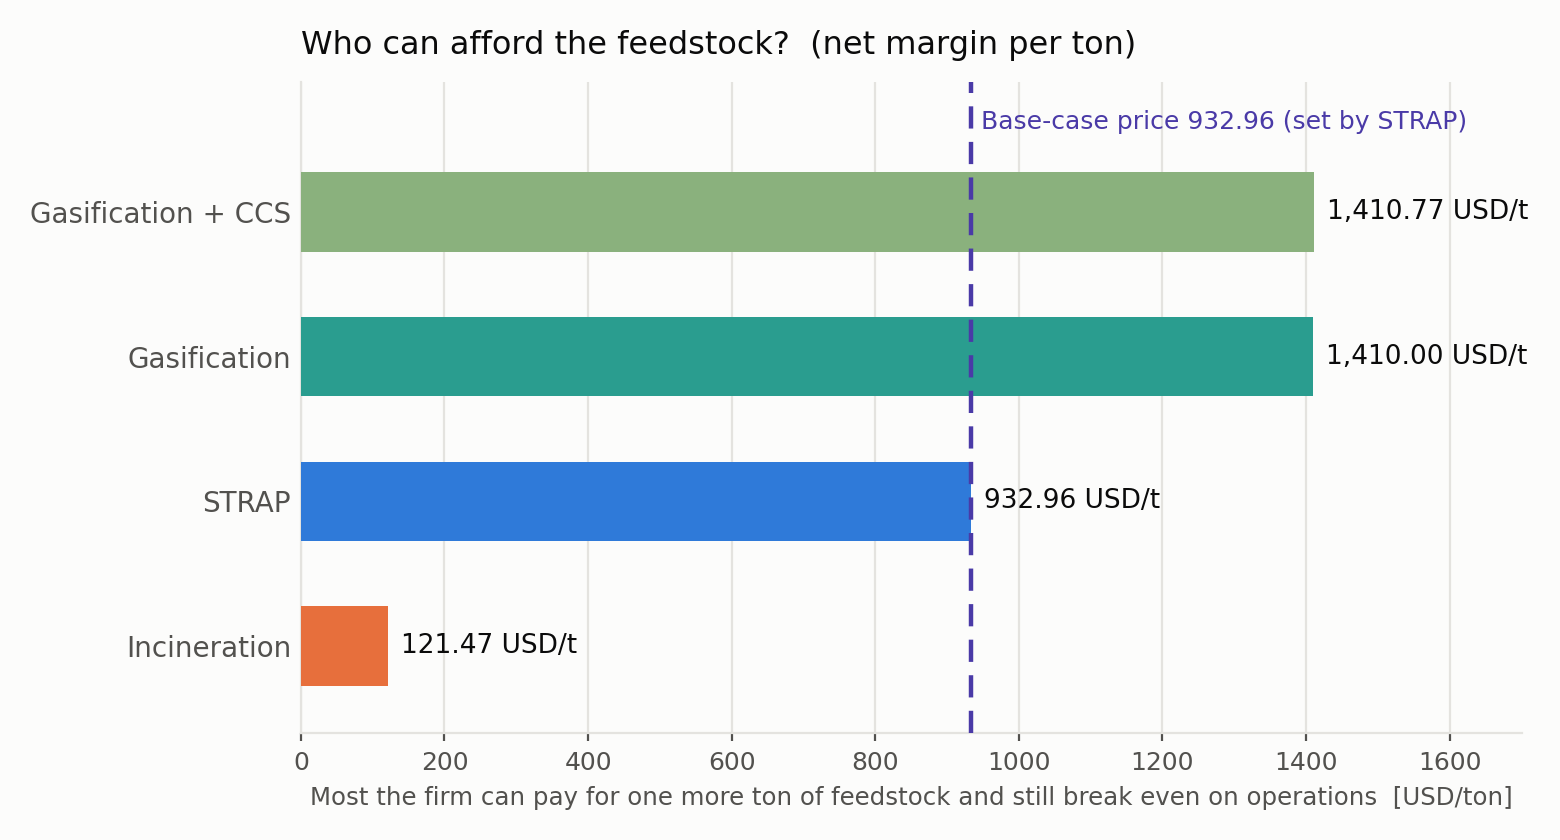
\includegraphics[width=0.88\textwidth]{fig1_margins.png}
\caption{Each firm's walk-away price. The dashed line is the equilibrium price at
20{,}000 t/yr: both gasification routes are above it, STRAP sits exactly on it, and
Incineration is far below.}
\label{fig:margins}
\end{figure}

\begin{readbox}
\textbf{Gasification and Gasification + CCS (1{,}410).} The two highest margins, and
almost identical. Without the credit, carbon capture would add 269 \usd/t of
operating cost (+120\%) for no revenue and leave CCS at 1{,}140.77, 270 \usd/t
behind. The 270 \usd/t credit cancels that extra cost to within 0.76 \usd/t, so CCS
comes out marginally \emph{ahead} (1{,}410.77 against 1{,}410.00). Both beat STRAP
by about 477 \usd/t.

\textbf{STRAP (932.96).} STRAP sells resin at a high price, but has the highest
operating cost of the four (535). It ranks third, which is what makes it the
price-setter at 20{,}000 t/yr.

\textbf{Incineration (121.47).} Energy is its only product. Its margin is
one-eighth of STRAP's, so it is the last resort: it gets waste only after every
other plant is full.
\end{readbox}

\begin{cautionbox}[title={The two gasification routes are nearly tied}]
Which one is ahead rests on 0.76 \usd/t. If the credit were any smaller than
269.24 \usd/t, plain Gasification would be first in the queue. This does not move the
base-case price, because both plants are full and STRAP sets it. It only decides
which of the two sets the price when the pool is below 16{,}000 t/yr, and there the
two candidate prices differ by 0.76 \usd/t. It is, however, why the credit's exact
value and basis are worth confirming (Q6).
\end{cautionbox}

\subsection{Base case: 20{,}000 t/yr}
\label{sec:base}

\textbf{Filling the queue.} Applying~\eqref{eq:closed}, the firms line up by margin:
\begin{enumerate}[leftmargin=1.6em,itemsep=0.1em]
  \item Gasification + CCS takes its full 8{,}000 t/yr. 12{,}000 t/yr remain.
  \item Gasification takes its full 8{,}000 t/yr. 4{,}000 t/yr remain.
  \item STRAP has room for 8{,}000 t/yr but only 4{,}000 remain. It is half filled
        and exactly on the margin, so it is the price-setter.
  \item Incineration gets nothing: the supply is used up.
\end{enumerate}
The price is therefore STRAP's margin:
\[
\boxed{\;\lambda^\ast = m_\strap = 1{,}468.39-535.43-0 = 932.96\ \usd/\text{ton}\;}
\]

\begin{table}[h]
\centering
\caption{Base-case equilibrium. Operating profit is margin $\times$ tons.}
\label{tab:base}
\begin{tabular}{@{}lrrlrrr@{}}
\toprule
Firm & Tons/yr & Share & State & Margin & $\mu_i$ & \shortstack{Operating\\profit (\usd/yr)} \\
\midrule
Gasification + CCS & 8{,}000 & 40\% & At capacity     & 1{,}410.77 & 477.81 & 11{,}286{,}125 \\
Gasification       & 8{,}000 & 40\% & At capacity     & 1{,}410.00 & 477.04 & 11{,}280{,}011 \\
STRAP              & 4{,}000 & 20\% & Price-setter    &    932.96  &   0    &  3{,}731{,}835 \\
Incineration       &       0 &  0\% & Priced out      &    121.47  &   0    &            0   \\
\midrule
Total & 20{,}000 & 100\% & & & & 26{,}297{,}971 \\
\bottomrule
\end{tabular}
\end{table}

\begin{readbox}
Four firms, three states (Table~\ref{tab:states}). The two gasification plants are
at capacity: they would take more waste if they could. STRAP is the price-setter:
half-filled, and the price is whatever makes it indifferent. Incineration is priced
out. The states carry the economics: ``at capacity'' means wants more,
``price-setter'' means indifferent, ``priced out'' means wants none.
\end{readbox}

\textbf{What $\lambda=932.96$ means.} It is the price of scarcity, and it is also the
most a waste generator could charge. If the generator charged $p_{\mathrm{raw}}$ per
ton, each firm's margin would fall by $p_{\mathrm{raw}}$ and $\lambda$ would fall by
the same amount, so the total a firm pays, $p_{\mathrm{raw}}+\lambda$, stays at
932.96. At $p_{\mathrm{raw}}=100$ the price is 832.96 and all 20{,}000 t/yr are still
sold. At 932.96 and above STRAP drops out and 4{,}000 t/yr go unsold; Gasification
drops out at 1{,}410.00 and Gasification + CCS at 1{,}410.77, after which nobody buys.

\begin{readbox}
932.96 is the generator's \emph{reservation price}. In the base case the generator
gives the waste away, so nobody pays $\lambda$, but the model says the generator
gives up as much as 932.96 \usd/t, about \usd{}18.7 million per year on 20{,}000 t.
Setting $p_{\mathrm{raw}}=0$ is therefore not neutral: it hands the whole price of
scarcity to the recyclers. A positive $p_{\mathrm{raw}}$ would share it between
generator and recyclers without changing the total cost to a recycler, as long as
all the waste is still sold. Section~\ref{sec:viabres} shows that the plants could not
actually afford to pay all of it.
\end{readbox}

\textbf{Where the profit comes from.} By~\eqref{eq:profit},
\[
\underbrace{26{,}297{,}971}_{\text{operating profit}}
=\underbrace{\lambda^\ast Q_{\mathrm{tot}}}_{932.96\times20{,}000\,=\,18{,}659{,}177}
+\underbrace{\textstyle\sum_i\mu_i\mathrm{Cap}_i}_{3{,}822{,}454\,+\,3{,}816{,}340\,=\,7{,}638{,}794}.
\]
The shadow prices are $\mu_\ccs=m_\ccs-m_\strap=477.81$ and
$\mu_\gas=m_\gas-m_\strap=477.04$ \usd/(t/yr).

\begin{readbox}
About 71\% of the operating profit is the value of the pile at the clearing price,
and 29\% is capacity rent earned by the two gasification plants. STRAP, as the
price-setter, earns no rent: its whole profit ($932.96\times4{,}000=3.73$ million)
is just the pile price on the tons it takes. The rent goes to the plants that are
full, not to the one that sets the price.

$\mu_\gas=477.04$ also means that moving one ton/yr of capacity from STRAP to
Gasification would add 477.04 \usd/yr to the system's operating profit; the same move
to Gasification + CCS adds 477.81, and to Incineration nothing.
\end{readbox}

\begin{cautionbox}[title={Not included in this result}]
\textbf{Emissions.} Without per-ton emission factors we cannot report system
emissions (Q9). Capital is treated in the next subsection.
\end{cautionbox}

\subsection{Profit after capital}
\label{sec:viabres}

Using~\eqref{eq:viab} with the annualized capital in Table~\ref{tab:inputs}:

\begin{table}[h]
\centering
\caption{Profit after capital at 20{,}000 t/yr. Incineration's capital was not
supplied, so it is not shown.}
\label{tab:viab}
\small
\begin{tabular}{@{}lrrrrr@{}}
\toprule
Firm & \shortstack{Operating\\profit} & \shortstack{Annualized\\capital} & \shortstack{Profit after\\capital} & \shortstack{Break-even\\tons/yr} & \shortstack{Break-even\\\% of capacity} \\
\midrule
Gasification + CCS & 11{,}286{,}125 & 7{,}077{,}509 &  4{,}208{,}615 & 5{,}017 & 63\% \\
Gasification       & 11{,}280{,}011 & 5{,}999{,}788 &  5{,}280{,}222 & 4{,}255 & 53\% \\
STRAP              &  3{,}731{,}835 & 6{,}314{,}456 & $-$2{,}582{,}620 & 6{,}768 & 85\% \\
\bottomrule
\end{tabular}
\end{table}

\begin{figure}[h]
\centering
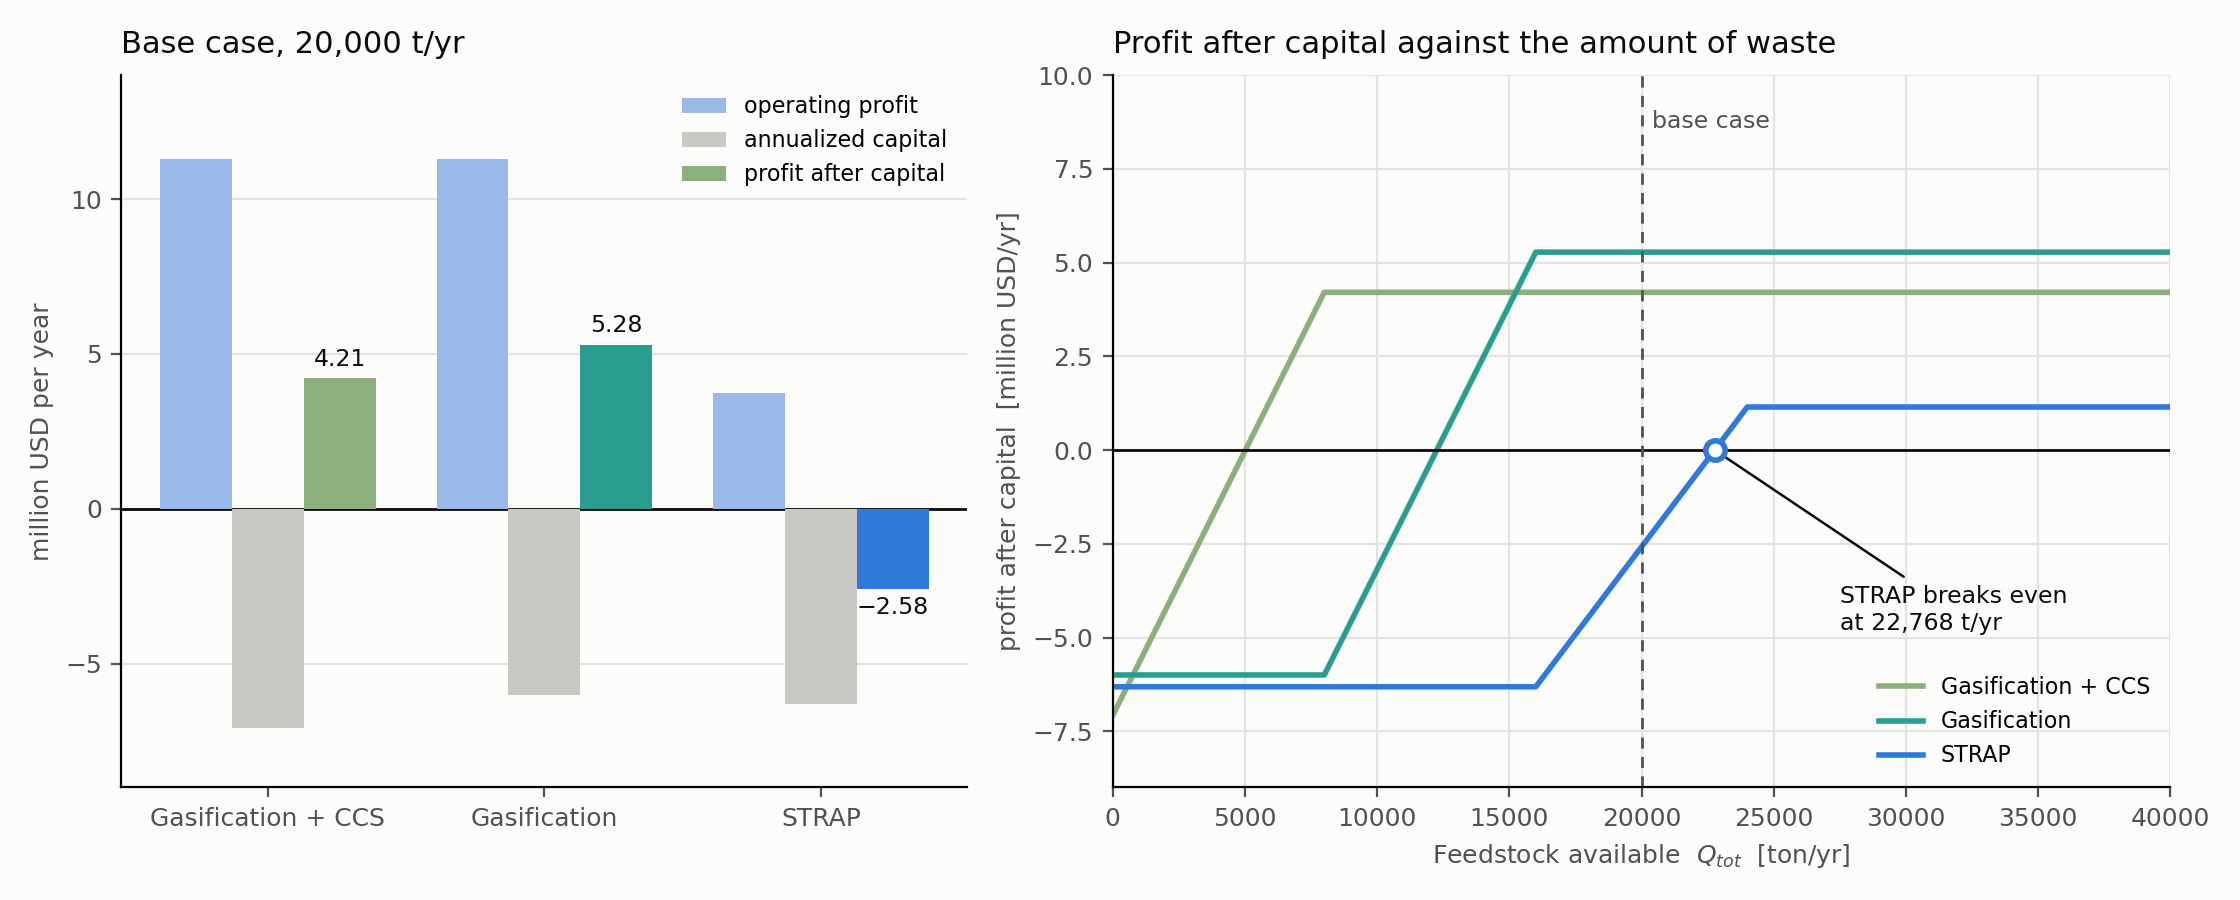
\includegraphics[width=0.98\textwidth]{fig6_profit.png}
\caption{Left: operating profit, annualized capital and profit after capital at the
base case. Right: profit after capital as the amount of waste varies. Each curve is
flat once its plant is full. STRAP only breaks even once the pool reaches
22{,}768 t/yr.}
\label{fig:profit}
\end{figure}

\begin{readbox}
\textbf{The two gasification plants pay back comfortably.} Each needs only about
half to two-thirds of its capacity to cover its capital, and each is full.

\textbf{STRAP does not.} It is the price-setter, so it gets only the 4{,}000 t/yr
left over, half its plant. Its operating profit of 3.73 million does not cover its
6.31 million capital charge, a loss of 2.58 million \usd/yr. STRAP needs 6{,}768 t/yr,
which in the queue means a pool of at least $16{,}000+6{,}768=22{,}768$ t/yr. Between
22{,}768 and 24{,}000 t/yr STRAP covers its capital \emph{and} the price is still
932.96.

\textbf{What happens if STRAP is not built.} The pool of 20{,}000 t/yr is then split
8{,}000 / 8{,}000 / 4{,}000 between the two gasification plants and Incineration, and
the price falls to Incineration's margin, 121.47 \usd/t (an 87\% drop). The
gasification plants' profits do not change, because the waste is free to them.

\textbf{The generator cannot capture the whole price.} Because the gasification
plants' capacity rent (about 3.8 million each) is less than their capital charge
(6.0 and 7.1 million), they only pay back because the waste is free. Each ton of
feedstock price takes 8{,}000 \usd/yr off a full plant. Gasification stays viable up
to $p_{\mathrm{raw}}=660$ \usd/t and Gasification + CCS up to 526 \usd/t, well below
the 932.96 reservation price.
\end{readbox}

\begin{cautionbox}[title={How to read this}]
The equilibrium of Section~\ref{sec:base} takes the plants as already built. The loss
for STRAP is a warning that, at 20{,}000 t/yr and these capacities, STRAP would not
have invested; it is not a change to the equilibrium itself. Incineration's capital is
not supplied (Q8), so the ``STRAP not built'' case treats the incinerator as already
built. Also, the break-even figures use the margin with the waste free; a positive
feedstock price raises each plant's break-even throughput.
\end{cautionbox}

\subsection{Price against the amount of waste}
\label{sec:sweep}

We re-solved the equilibrium for pools from 0 to 40{,}000 t/yr (209 points,
including each threshold and points just either side).

\begin{figure}[h]
\centering
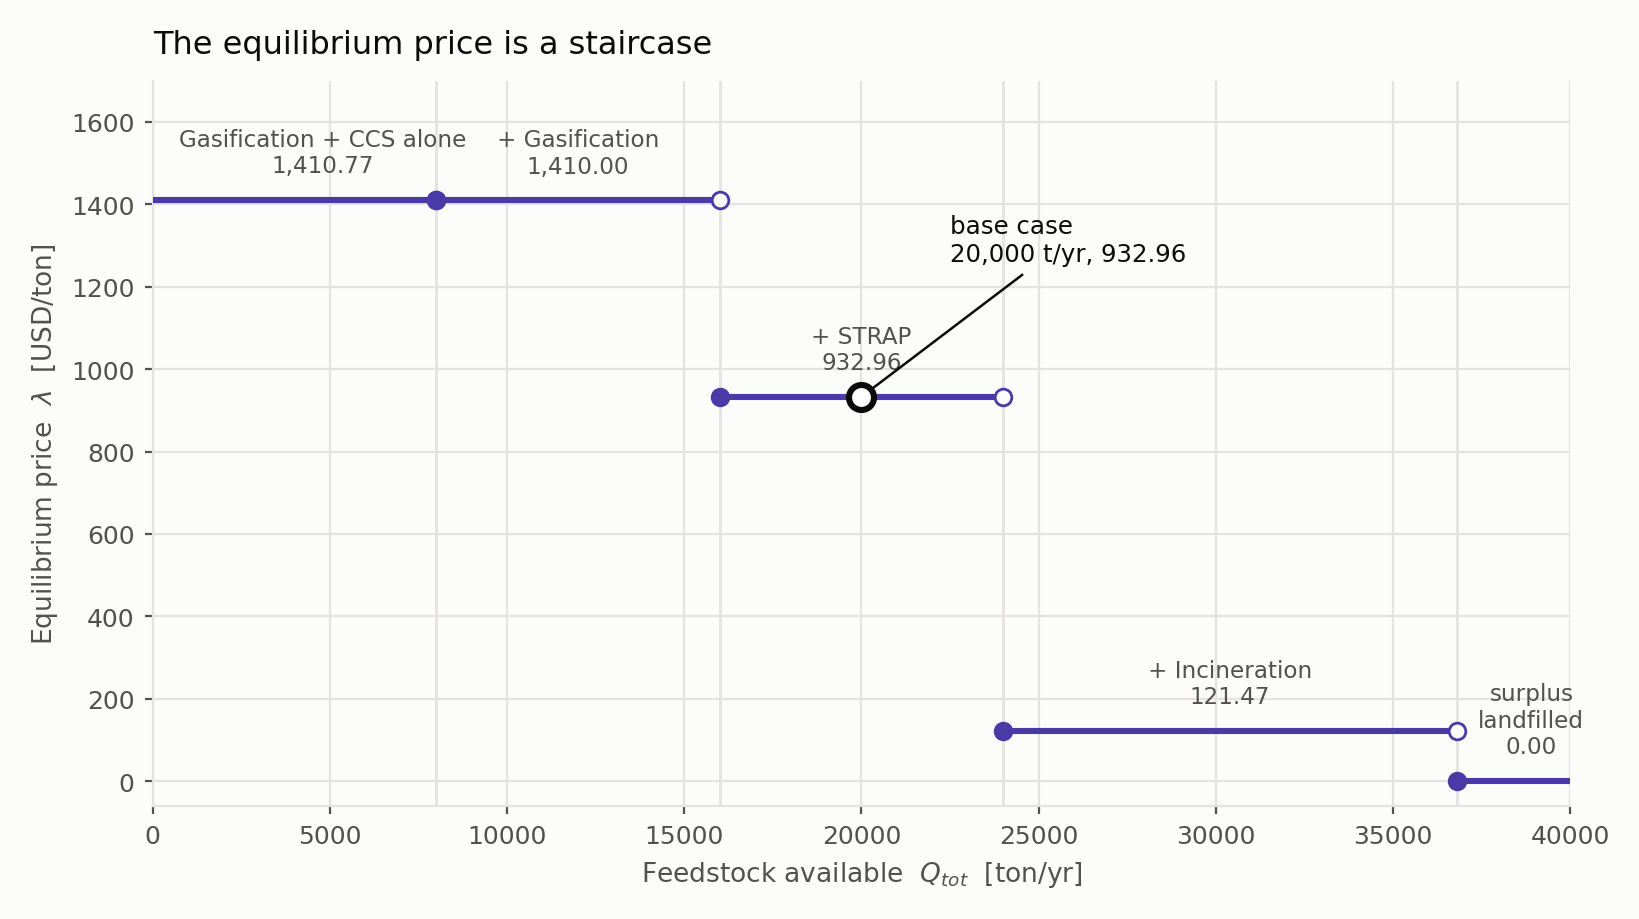
\includegraphics[width=0.88\textwidth]{fig2_staircase.png}
\caption{Equilibrium price against the amount of waste: a staircase, flat within a
step with a jump each time the price-setter changes. Filled dots are the reported
(lowest) price at each threshold.}
\label{fig:stairs}
\end{figure}

\begin{table}[h]
\centering
\caption{The five steps of the price, from~\eqref{eq:closed}.}
\label{tab:regimes}
\small
\begin{tabular}{@{}llrl@{}}
\toprule
Waste (t/yr) & Who is buying & $\lambda$ (\usd/t) & Price-setter ($=\lambda$) \\
\midrule
below 8{,}000        & Gasification + CCS only          & 1{,}410.77 & Gasification + CCS, $m_\ccs$ \\
8{,}000 to 16{,}000  & + Gasification                   & 1{,}410.00 & Gasification, $m_\gas$ \\
16{,}000 to 24{,}000 & + STRAP \textbf{(base case)}     &    932.96  & STRAP, $m_\strap$ \\
24{,}000 to 36{,}800 & + Incineration                   &    121.47  & Incineration, $m_\inc$ \\
above 36{,}800       & all full; surplus landfilled     &      0     & nobody \\
\bottomrule
\end{tabular}
\end{table}

The thresholds are the running totals $K_k$ of the capacities in queue order:
8{,}000, 16{,}000 and 24{,}000, then $24{,}000+12{,}800=36{,}800$.

\begin{readbox}
The staircase is the demand curve for waste read sideways. While the pile is smaller
than the first plant's capacity, that plant alone absorbs everything and the price is
its margin. Once the pile is bigger, the leftover goes to the next firm and the price
drops to \emph{that} firm's margin. Once the pile exceeds every plant, the surplus
has no buyer and the price is zero. The model gives the step, and the step sets the
price. Within a step, a ton more or less changes nothing.
\end{readbox}

\begin{figure}[h]
\centering
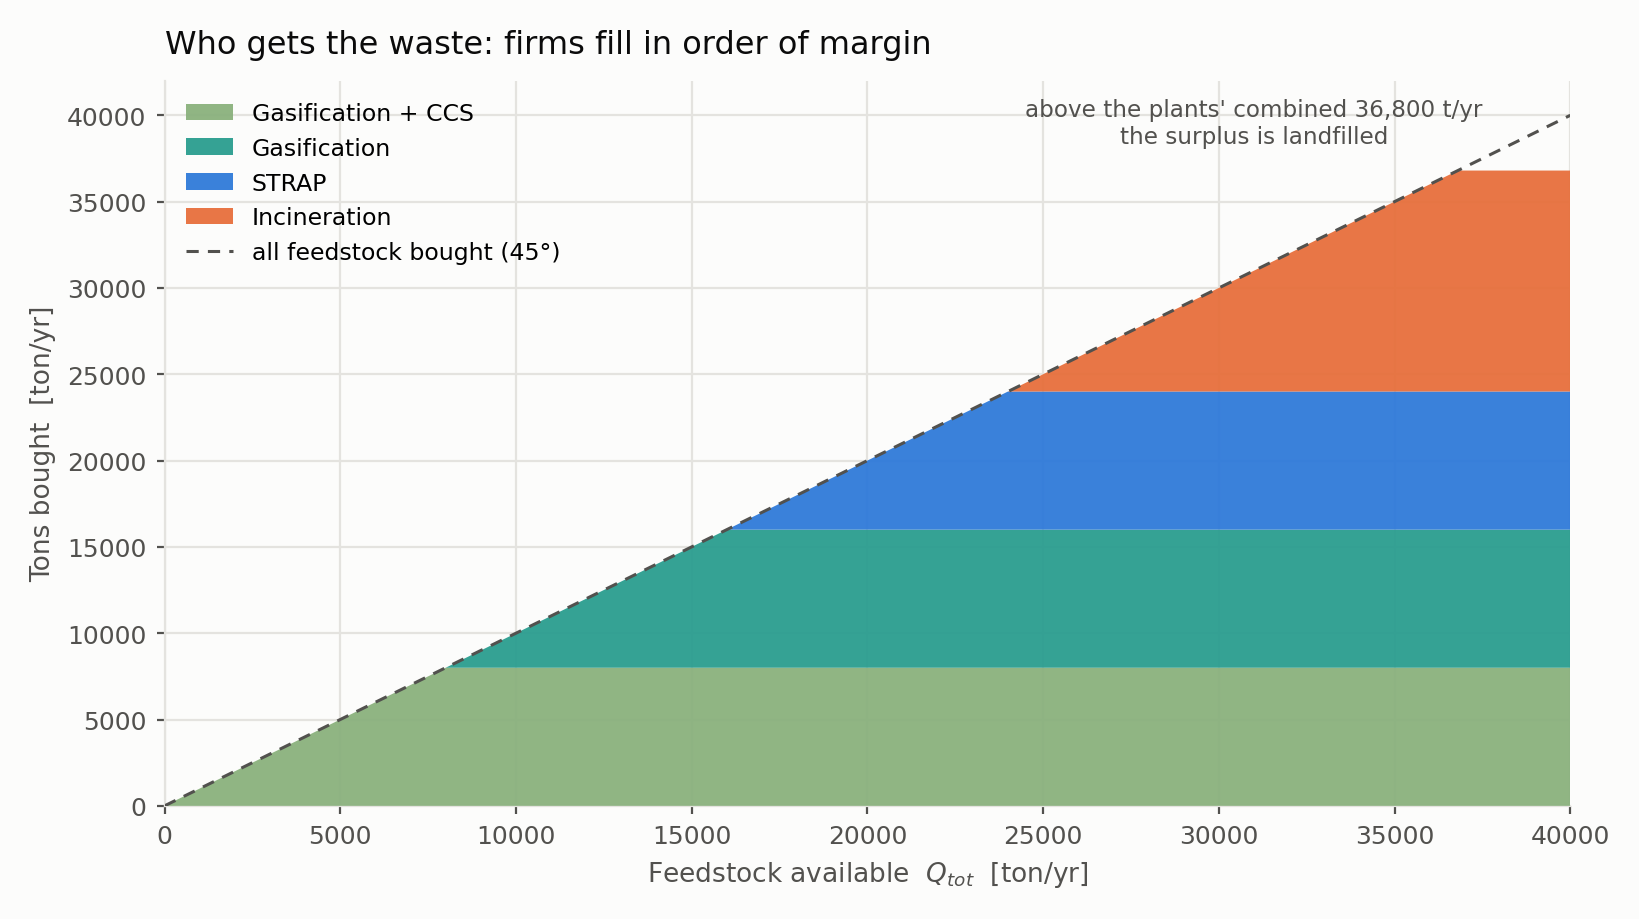
\includegraphics[width=0.88\textwidth]{fig3_allocation.png}
\caption{Who gets the waste. Gasification + CCS fills first, then Gasification, then
STRAP, then Incineration. Above 36{,}800 t/yr the gap to the dashed line is waste
nobody buys.}
\label{fig:alloc}
\end{figure}

\textbf{The drops are very uneven.} The price falls by only 0.76 \usd/t at 8{,}000
(the near-tie between the two gasification routes), by 477 (34\%) at 16{,}000, and by
\textbf{811 (87\%)} at 24{,}000. The small drop is between the two gasification
routes; the large ones are from gasification down to STRAP and from STRAP down to
Incineration. The same shows up in the total implicit value of the pile,
$\lambda Q_{\mathrm{tot}}$: about 18.7 million \usd{} at 20{,}000 t/yr, 22.4 million
just below 24{,}000, then 2.9 million just above and 3.6 million at 30{,}000. A bigger
pile can be worth much less in total, because the extra waste goes to a buyer who
values it far less.

\textbf{At the thresholds the price is not unique.} At exactly 8{,}000, 16{,}000,
24{,}000 and 36{,}800 t/yr, any price between the two adjacent steps is consistent
with equilibrium. We report the lowest. A drop should be read as ``just below versus
just above'', not as the response to one extra ton.

\begin{readbox}
\textbf{The base case is not on a knife edge.} At 20{,}000 t/yr we are 4{,}000 t
inside each edge of the STRAP step. The pile could be 20\% smaller or 20\% larger
and the price would still be 932.96, with the same three firms buying.

\textbf{What this can and cannot tell us.} The order of firms and the thresholds
depend only on the margins and capacities. The model cannot show a \emph{gradient}:
at 17{,}000 and at 23{,}000 t/yr it returns the same price. With constant cost per
ton it describes scarcity steps, not ``a little scarcer''. A convex-cost version
would give a sloped price and is the natural next step.
\end{readbox}

\subsection{Sensitivity}
\label{sec:sensitivity}

\textbf{Why the price depends on STRAP.} With these capacities, the best two firms
together (16{,}000 t/yr) cannot cover 20{,}000 t/yr but the best three (24{,}000)
can. By~\eqref{eq:closed} the third firm in the queue is price-setter:
\[
\lambda^\ast=\text{third-highest margin}=m_\strap=932.96 .
\]
We verified this rule on 1{,}527 random sets of margins.

\begin{table}[h]
\centering
\caption{Effect on $\lambda$ at 20{,}000 t/yr of changing one input, all else at the
base case. A flip point is where the ranking of firms changes.}
\label{tab:sens}
\small
\renewcommand{\arraystretch}{1.2}
\begin{tabular}{@{}>{\raggedright\arraybackslash}p{3.7cm}>{\raggedright\arraybackslash}p{2.6cm}>{\raggedright\arraybackslash}p{8.6cm}@{}}
\toprule
\textbf{Input} & \textbf{Change} & \textbf{Effect on $\lambda$} \\
\midrule
STRAP revenue & $+1$ \usd/t & $+1$ (one-for-one) while revenue is between 656.90 and 1{,}945.43 ($-55\%$ to $+32\%$). Above 1{,}945.43, STRAP overtakes Gasification and $\lambda=1{,}410.00$. Below 656.90, STRAP falls below Incineration and $\lambda=121.47$. \\
STRAP operating cost & $+1$ \usd/t & $-1$ (one-for-one) while cost is between 58.38 and 1{,}346.92 ($-89\%$ to $+152\%$). \\
Feedstock price $p_{\mathrm{raw}}$ & $+1$ \usd/t & $-1$ (one-for-one); $\lambda=0$ at 932.96, where STRAP drops out. \\
Gasification + CCS revenue or cost & any, within limits & None, until its margin falls below STRAP's: revenue below 1{,}427.19 ($-25.1\%$ from 1{,}905) or cost above 972.04 ($+97\%$). Then $\lambda=m_\ccs$, one-for-one. The credit alone cannot trigger this: with no credit at all the margin is still 1{,}140.77. \\
Gasification revenue or cost & any, within limits & None, until its margin falls below STRAP's: revenue below 1{,}157.96 ($-29.2\%$) or cost above 702.04 ($+212\%$). \\
Incineration revenue or cost & any, within limits & None, unless its margin rises above STRAP's: revenue above 1{,}071.06, over four times today's 259.57. \\
Plant capacities & see Figure~\ref{fig:regime} & Jumps between 1{,}410.00, 932.96 and 121.47. \\
Capital cost & any & None. Changes profit after capital only. \\
\bottomrule
\end{tabular}
\end{table}

\begin{readbox}
\textbf{Three kinds of input.}
\emph{(i)~STRAP's own numbers} move the price one-for-one, because STRAP \emph{is} the
price now. A 10\% error in STRAP's operating cost (54 \usd/t) is a 54 \usd/t error in
$\lambda$, and a 10\% error in its revenue (147 \usd/t) a 147 \usd/t error.
\emph{(ii)~Capacities} do not shift the price smoothly. They decide which step we are
in, so a wrong capacity either changes nothing or changes a lot.
\emph{(iii)~The gasification and incineration numbers, and the CCS credit,} do not
matter at this pile size as long as those firms keep their places in the queue. The
flip points say how wrong they would have to be to matter. Gasification + CCS is the
most exposed: a 25\% drop in its revenue is enough.
\end{readbox}

\begin{figure}[h]
\centering
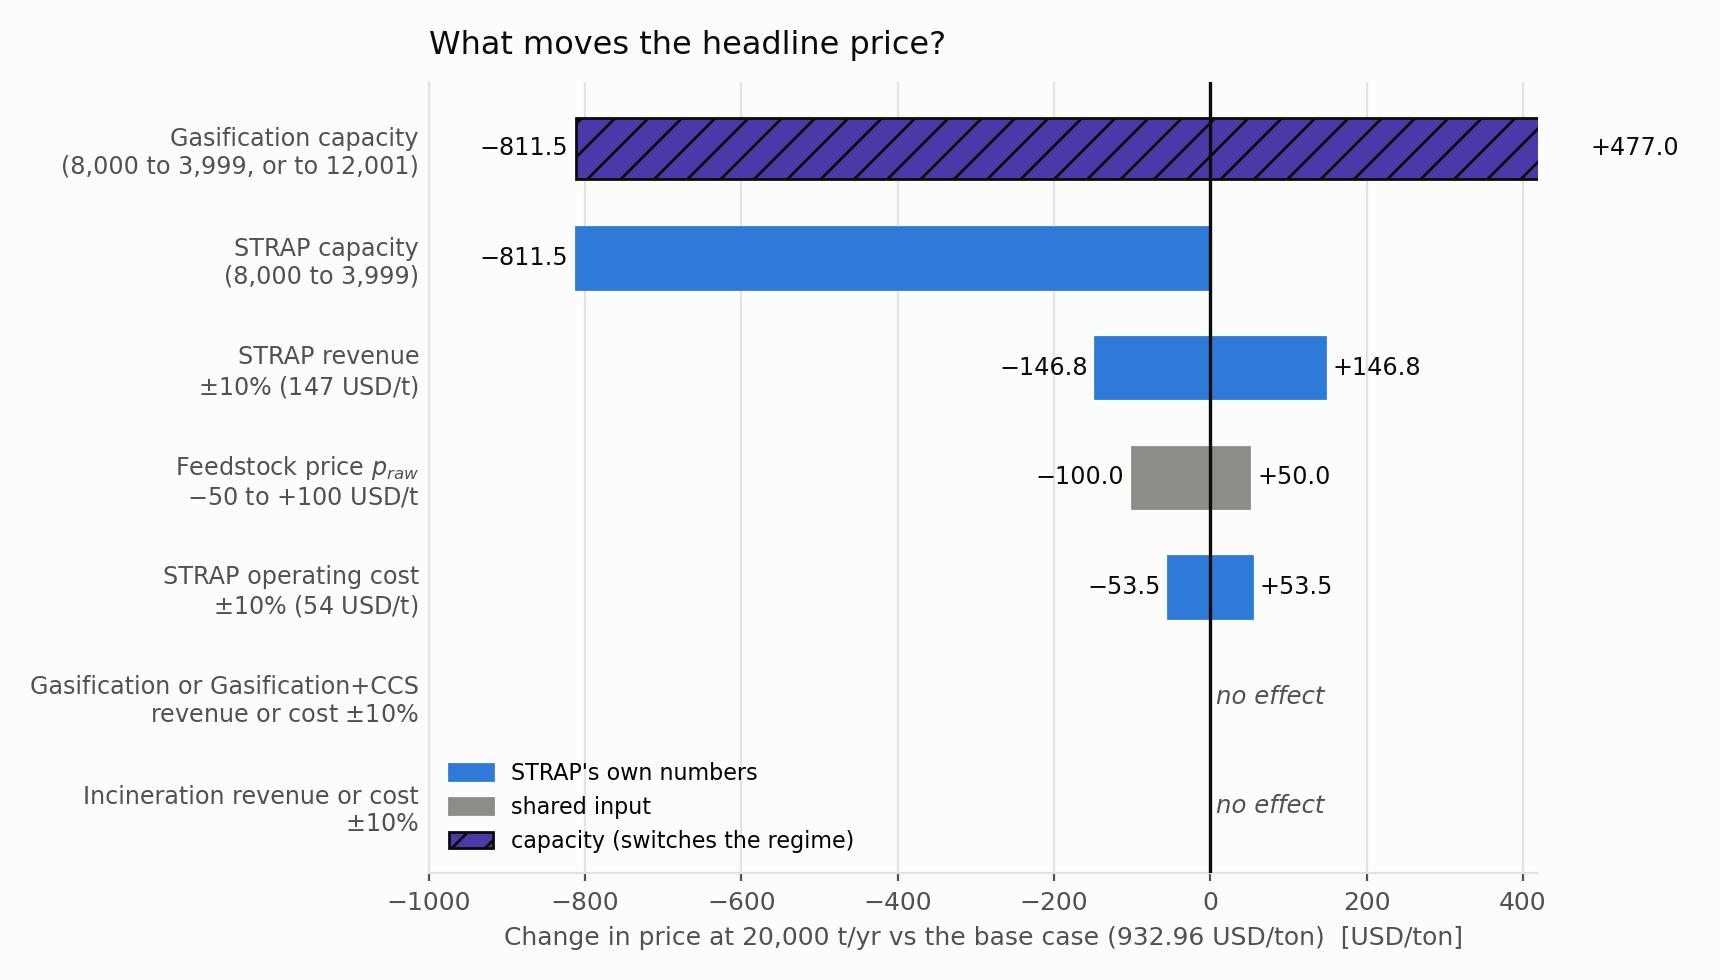
\includegraphics[width=0.92\textwidth]{fig4_tornado.png}
\caption{Change in $\lambda$ at 20{,}000 t/yr when each input is moved, all else at
the base case. Capacities dominate because they switch the step. Among smooth
inputs, STRAP's revenue and the feedstock price matter most.}
\label{fig:tornado}
\end{figure}

\begin{figure}[h]
\centering
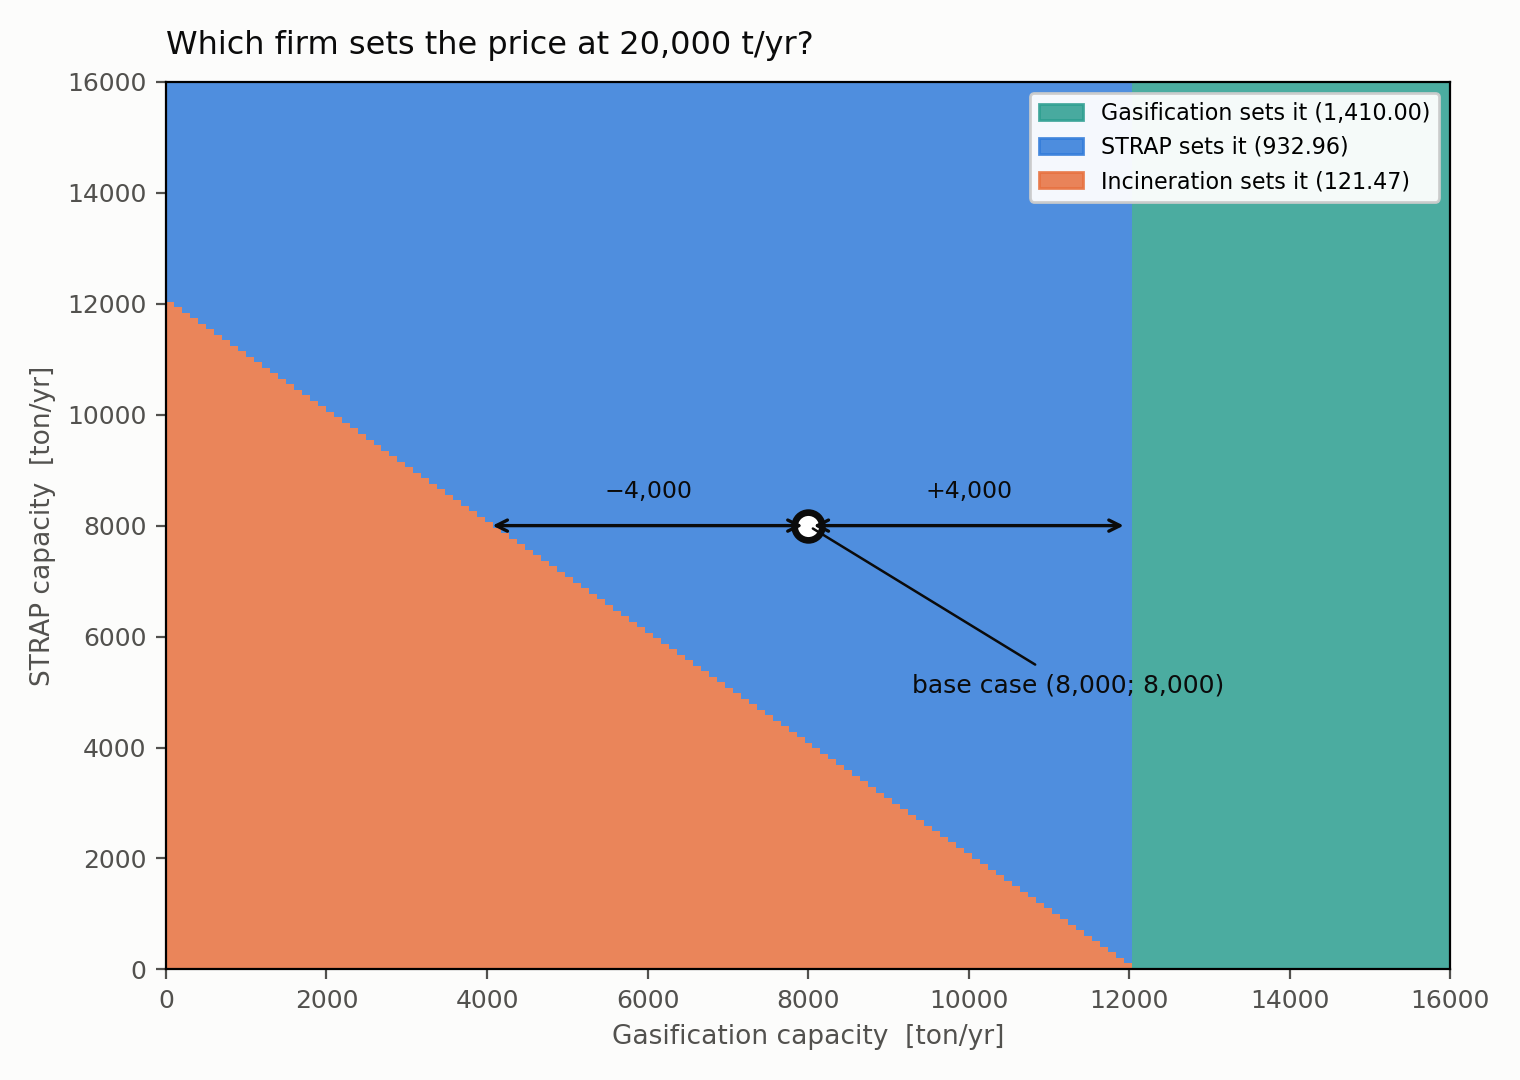
\includegraphics[width=0.85\textwidth]{fig5_regime_map.png}
\caption{Which firm sets the price at 20{,}000 t/yr as the Gasification and STRAP
capacities vary (Gasification + CCS at 8{,}000 and Incineration at 12{,}800 held
fixed). The base case is the white dot. Colors come from solving the model at each
point.}
\label{fig:regime}
\end{figure}

\begin{readbox}
Figure~\ref{fig:regime} shows how wrong the capacity assumptions can be before the
price jumps. From (8{,}000; 8{,}000):
\begin{itemize}[leftmargin=1.4em,itemsep=0.15em,topsep=0.2em]
  \item The Gasification capacity can \textbf{fall by 4{,}000} or \textbf{rise by
        4{,}000}. Fall further and Incineration becomes the price-setter ($\lambda$
        drops from 932.96 to 121.47). Rise further and Gasification itself becomes
        the price-setter ($\lambda$ rises to 1{,}410.00).
  \item STRAP's capacity can rise without limit but cannot fall below 4{,}000;
        below that, STRAP is full and Incineration sets the price.
\end{itemize}
STRAP is the price-setter exactly when the two plants ahead of it hold less than
20{,}000 t/yr together and the three together hold at least 20{,}000. The capacities
are assumed, so this $\pm$4{,}000 t/yr margin is what to keep in mind when reading
the headline.
\end{readbox}

% =============================================================================
\section{Discussion}
\label{sec:discussion}

\subsection{Limitations}
\label{sec:limits}

\begin{itemize}[leftmargin=1.4em,itemsep=0.25em]
  \item \textbf{Linear operating cost.} Cost per ton is constant. This is what makes
        the price a staircase. A convex-cost version would give a smoothly varying
        price and a unique split of waste.
  \item \textbf{Fixed prices.} Hydrogen, resin and energy prices are inputs. In
        reality, if the gasification plants sold much more hydrogen the price would
        fall, and their margin with it.
  \item \textbf{No cost coupling.} The feedstock price does not depend on how much
        any firm buys, and landfill is free to the firms. Coupling them would
        break the equivalence with the planner's problem.
  \item \textbf{Fixed capacities, capital as a check.} Plant sizes are inputs, not the
        outcome of a capacity-choice game, and capital enters profit but not the
        equilibrium. Section~\ref{sec:viabres} shows STRAP would not break even at
        these capacities, so a game in which firms choose whether to build would give
        a different answer. A plant earning capacity rent (here the two gasification
        plants) also has an incentive to grow.
  \item \textbf{Incineration capital and emissions are missing.} See Q8 and Q9.
\end{itemize}

\subsection{Verification}

Every check is in \texttt{Code/check.py}; it exits with an error if any fails, and
all passed.
\begin{enumerate}[leftmargin=1.6em,itemsep=0.15em]
  \item \textbf{Margins} re-typed from Paola's table (with the 270 credit), without
        the model code, match to $10^{-9}$.
  \item \textbf{Planner LP.} Solving~\eqref{eq:planner} as a linear program gives the
        same 8{,}000 / 8{,}000 / 4{,}000 / 0 split, with dual values exactly
        $\lambda=932.96$, $\mu_\ccs=477.81$ and $\mu_\gas=477.04$.
  \item \textbf{Brute force.} For each of the 209 sweep points we scanned candidate
        prices and took the lowest at which demand fits; it matches the model at all
        209. The LP split also matches away from the thresholds.
  \item \textbf{KKT.} All conditions~\eqref{eq:kkt1}--\eqref{eq:kkt3} hold with a
        worst violation of exactly zero (the solution is closed-form).
  \item \textbf{Shape.} The price never rises as the pool grows, takes exactly five
        values, switches at 8{,}000 / 16{,}000 / 24{,}000 / 36{,}800 t/yr, and no two
        firms tie on margin.
  \item \textbf{Identities.} \eqref{eq:profit} holds
        ($26{,}297{,}971=18{,}659{,}177+7{,}638{,}794$), and the third-highest-margin
        rule holds on 1{,}527 random margin sets.
  \item \textbf{Random problems.} On 3{,}000 random four-firm problems, the solver's
        allocation, price and KKT conditions agree with the LP.
  \item \textbf{Capital.} Profit after capital and break-even tons for the three
        firms with capital data were recomputed from the raw table, STRAP's break-even
        pool (22{,}768 t/yr) matches the solver on either side, incineration's missing
        capital is reported as missing and not as zero, and adding the capital
        constants to the planner's objective leaves its allocation unchanged.
\end{enumerate}
These checks show that the code and algebra are right, not that the inputs are. The
answer is only as good as STRAP's operating cost, the capacities and the pool size.

% =============================================================================
\subsection{Questions for Paola}
\label{sec:questions}

Each question lists what we assumed and what the answer would change. The effect is
computed at 20{,}000 t/yr with everything else at the base case.

{\small
\setlength{\tabcolsep}{4pt}
\renewcommand{\arraystretch}{1.25}
\begin{longtable}{@{}>{\raggedright\arraybackslash}p{0.5cm}>{\raggedright\arraybackslash}p{6.2cm}>{\raggedright\arraybackslash}p{3.3cm}>{\raggedright\arraybackslash}p{4.6cm}@{}}
\toprule
 & \textbf{What we need from you} & \textbf{What we assumed} & \textbf{Effect on $\lambda$} \\
\midrule
\endhead
\multicolumn{4}{@{}l}{\textbf{Move the headline price directly}}\\*[0.2em]
1 & \textbf{Size of the waste pool.} How much post-industrial multilayer film is available per year to these four plants? & 20{,}000 t/yr \ASSUMED, chosen so the firms genuinely compete & Steps at 8{,}000, 16{,}000, 24{,}000 and 36{,}800 t/yr (Table~\ref{tab:regimes}). Anywhere in 16{,}000--24{,}000 gives 932.96. STRAP covers its capital only above 22{,}768 t/yr. \\
2 & \textbf{Plant capacities.} Are the plant sizes right? Is there a defensible single-plant size for STRAP (its 8{,}000 t/yr plant runs half empty at 20{,}000 t/yr and loses money), and is 12{,}800 t/yr the right Incineration capacity? & 8{,}000 each for Gasification, Gasification + CCS and STRAP; 12{,}800 for Incineration \ASSUMED & Jumps between 1{,}410.00, 932.96 and 121.47. The base case tolerates $\pm$4{,}000 t/yr on the Gasification capacity (Figure~\ref{fig:regime}). \\
3 & \textbf{STRAP operating cost.} We read 535.43 \usd/t as the all-in operating cost including landfilling STRAP's residue, with no capital. Is that right? & 535.43 \usd/t \PAOLA\ (our reading of ``with landfill'') & One-for-one: $\pm$10\% gives $\mp$53.5. \\
4 & \textbf{STRAP revenue.} Is 1{,}468.39 \usd/t still right, on the same price basis as the gasification revenue? & 1{,}468.39 \usd/t \PAOLA & One-for-one: $\pm$10\% gives $\pm$146.8. \\
5 & \textbf{Feedstock price.} What does the waste generator charge, if anything? It could be negative (the generator pays to offload it). & 0 \usd/t \ASSUMED & $-1$ per dollar; $-50$ gives 982.96, $+100$ gives 832.96. Gasification stops covering its capital above 660 \usd/t and CCS above 526. \\[0.4em]
\midrule
\multicolumn{4}{@{}l}{\textbf{Change the ranking or the story}}\\*[0.2em]
6 & \textbf{The 45Q credit.} Is 270 \usd{} per ton of \emph{feed} (not per ton of CO$_2$ captured), how many years does it last, and is it net of transport and storage costs? & 270 \usd/t added to CCS revenue \PAOLA & None at 20{,}000 t/yr. CCS and Gasification are tied to within 0.76 \usd/t: a credit below 269.24 puts Gasification first. At 8{,}000--16{,}000 t/yr it changes the price by at most 0.76. \\
7 & \textbf{Hydrogen revenue.} How is 1{,}635 \usd/t built (hydrogen yield $\times$ price), and is it the same for the CCS route? & 1{,}635 for both \PAOLA & None unless it falls by 25.1\% (CCS) or 29.2\% (Gasification). \\[0.4em]
\midrule
\multicolumn{4}{@{}l}{\textbf{Do not change $\lambda$, but are needed for a full analysis}}\\*[0.2em]
8 & \textbf{Incineration capital, and the capital basis.} What is Incineration's annualized capital? Also, is the ``MM USD'' figure per year for the plant sizes quoted, and how does capital change if a plant is a different size (for example STRAP at 4{,}000 t/yr)? & Incineration: not included. Others: as supplied \PAOLA & None. Changes profit after capital, and whether Incineration is viable when STRAP is not built. \\
9 & \textbf{Emissions.} Per-ton process emissions for each technology (with the capture rate for CCS), and the landfill factor for unbought waste. & Not included & None. Needed to report emissions. \\
10 & \textbf{Scale of the cost figures.} Gasification and STRAP costs are for an 8{,}000 t/yr plant and Incineration's for a 100{,}000 t/yr plant. Is it fair to hold them constant per ton at the capacities used? & Constant per ton \ASSUMED & None while cost per ton is unchanged; a scale effect would change margins. \\
\bottomrule
\end{longtable}
}

\begin{readbox}
If there is time for only three questions, ask \textbf{3, 2 and 1}: STRAP's operating
cost is the price (Q3), and the capacities and pool size decide which step we are in
(Q2, Q1) and whether STRAP pays back. Next come Q6 (the credit that holds the two
gasification routes level) and Q8 (Incineration capital, needed to finish the
viability analysis).
\end{readbox}

% =============================================================================
\appendix
\section{Reproducing the results}

All commands are run from \texttt{Paola\_Game\_Theory/Code/}.
\begin{center}
\small
\renewcommand{\arraystretch}{1.2}
\begin{tabular}{@{}ll@{}}
\toprule
\textbf{What} & \textbf{File or command} \\
\midrule
Inputs (including the credit and capital) & \texttt{data.py} \\
Solver, profits and break-even & \texttt{solver.py} \\
Figures 1--6 and \texttt{results/sweep\_q\_tot.csv} & \texttt{python plots.py} \\
All checks in Section~\ref{sec:discussion} & \texttt{python check.py} \\
\bottomrule
\end{tabular}
\end{center}

\section*{References}
\begin{flushleft}
\noindent Mu\~{n}oz-Briones, Ikegwu, Martinez, Granger, Van Lehn, Zavala, Huber and
Avraamidou. \emph{Decision support for circular economy waste management of mixed
plastic streams: A case study on post-industrial multilayer films.}

\medskip
\noindent Global CCS Institute. \emph{U.S.\ Preserves and Increases 45Q Credit in
``One Big Beautiful Bill Act''}. 2025.
\url{https://www.globalccsinstitute.com/u-s-preserves-and-increases-45q-credit-in-one-big-beautiful-bill-act/}
\end{flushleft}

\end{document}
